\documentclass[]{article}
\usepackage{lmodern}
\usepackage{amssymb,amsmath}
\usepackage{ifxetex,ifluatex}
\usepackage{fixltx2e} % provides \textsubscript
\ifnum 0\ifxetex 1\fi\ifluatex 1\fi=0 % if pdftex
  \usepackage[T1]{fontenc}
  \usepackage[utf8]{inputenc}
\else % if luatex or xelatex
  \ifxetex
    \usepackage{mathspec}
  \else
    \usepackage{fontspec}
  \fi
  \defaultfontfeatures{Ligatures=TeX,Scale=MatchLowercase}
\fi
% use upquote if available, for straight quotes in verbatim environments
\IfFileExists{upquote.sty}{\usepackage{upquote}}{}
% use microtype if available
\IfFileExists{microtype.sty}{%
\usepackage{microtype}
\UseMicrotypeSet[protrusion]{basicmath} % disable protrusion for tt fonts
}{}
\usepackage[margin=1in]{geometry}
\usepackage{hyperref}
\hypersetup{unicode=true,
            pdftitle={LuteinizingHormone},
            pdfauthor={Katie},
            pdfborder={0 0 0},
            breaklinks=true}
\urlstyle{same}  % don't use monospace font for urls
\usepackage{graphicx,grffile}
\makeatletter
\def\maxwidth{\ifdim\Gin@nat@width>\linewidth\linewidth\else\Gin@nat@width\fi}
\def\maxheight{\ifdim\Gin@nat@height>\textheight\textheight\else\Gin@nat@height\fi}
\makeatother
% Scale images if necessary, so that they will not overflow the page
% margins by default, and it is still possible to overwrite the defaults
% using explicit options in \includegraphics[width, height, ...]{}
\setkeys{Gin}{width=\maxwidth,height=\maxheight,keepaspectratio}
\IfFileExists{parskip.sty}{%
\usepackage{parskip}
}{% else
\setlength{\parindent}{0pt}
\setlength{\parskip}{6pt plus 2pt minus 1pt}
}
\setlength{\emergencystretch}{3em}  % prevent overfull lines
\providecommand{\tightlist}{%
  \setlength{\itemsep}{0pt}\setlength{\parskip}{0pt}}
\setcounter{secnumdepth}{0}
% Redefines (sub)paragraphs to behave more like sections
\ifx\paragraph\undefined\else
\let\oldparagraph\paragraph
\renewcommand{\paragraph}[1]{\oldparagraph{#1}\mbox{}}
\fi
\ifx\subparagraph\undefined\else
\let\oldsubparagraph\subparagraph
\renewcommand{\subparagraph}[1]{\oldsubparagraph{#1}\mbox{}}
\fi

%%% Use protect on footnotes to avoid problems with footnotes in titles
\let\rmarkdownfootnote\footnote%
\def\footnote{\protect\rmarkdownfootnote}

%%% Change title format to be more compact
\usepackage{titling}

% Create subtitle command for use in maketitle
\newcommand{\subtitle}[1]{
  \posttitle{
    \begin{center}\large#1\end{center}
    }
}

\setlength{\droptitle}{-2em}

  \title{LuteinizingHormone}
    \pretitle{\vspace{\droptitle}\centering\huge}
  \posttitle{\par}
    \author{Katie}
    \preauthor{\centering\large\emph}
  \postauthor{\par}
      \predate{\centering\large\emph}
  \postdate{\par}
    \date{February 1, 2019}


\begin{document}
\maketitle

\section{Background}\label{background}

The luteinizing hormone (LH) necessitates fertility in humans. Female
ovulation is induced by a rapid surge of LH, which can be measured by
analyzing blood samples. Understanding changes in LH levels during
ovulation could be useful in assessing a woman's fertility and
potentially guiding conception.

\section{Problem}\label{problem}

A female patient has provided a series of blood samples from which the
LH levels have been measured.The goal of this activity was to analyze
changes in LH hormone levels during ovulation through answering the
following questions:

\begin{itemize}
\tightlist
\item
  Is the LH hormone level over time a stationary process?
\item
  Does a suitable model exist that could be used to predict future
  hormone levels?
\item
  If a model exists, what is the equation for the model?
\end{itemize}

\section{Data Source}\label{data-source}

The data were obtained from library(datasets) in R, but was was
originally released in a Biostatistical reference book (Diggens, 1990).
The data set contains 48 samples at 10-minute intervals that were
obtained from the female patient.

\section{Exploring Data \& Assessing
Stationarity}\label{exploring-data-assessing-stationarity}

The data were visualized in a time series plot, as shown below. The
autocorrelations were also plotted in order to assess stationarity. The
plots were examined to determine if the behavior was consistent with
that of any known classes of time series models, such as the
autoregressive or moving average models.

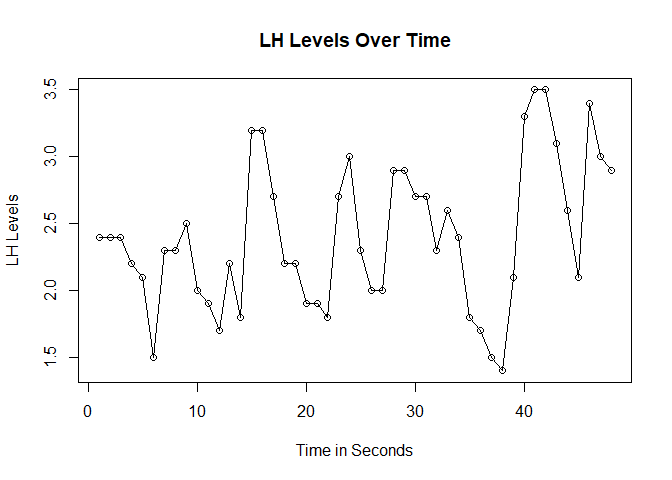
\includegraphics{LH_TS_files/figure-latex/lh-1.pdf}
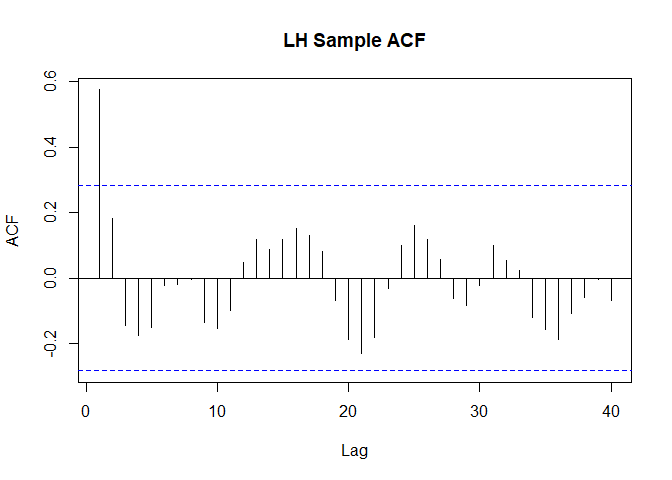
\includegraphics{LH_TS_files/figure-latex/lh-2.pdf}

The autocorrelations at various lags were plotted, as shown in the
correlogram above. The autocorrelation appeared to decay after the first
lag, remaining within the confidence bounds thereafter. The apparent
lack of dependence of the ACF on time is consistent with stationarity.
Furthermore, the series did not appear to exhibit any strong or
persistant trends, aside from a few peaks and valleys, that would have
suggested a non-constant mean or variance.

In terms of candidate models, an autocorrelation that decays after the
first lag could suggest a first order moving average. However, it is
also possible that the series could be autoregressive, if the slight
oscillations contained within the confidence bounds of the correlogram
are not regarded as insignificant. It is conceivable that these
autocorrelations are simply \emph{close}, but not necessarily equal, to
zero. If that is the case, then the ACF could be interpreted as
``tailing off'' rather than ``dying out'', which would be more
consistent with the expected behavior for an autoregressive series.

To test these theories, the partial acf should also be generated,
plotted, and examined. The pacf behavior should then be compared to the
general expectations for both AR and MA models.

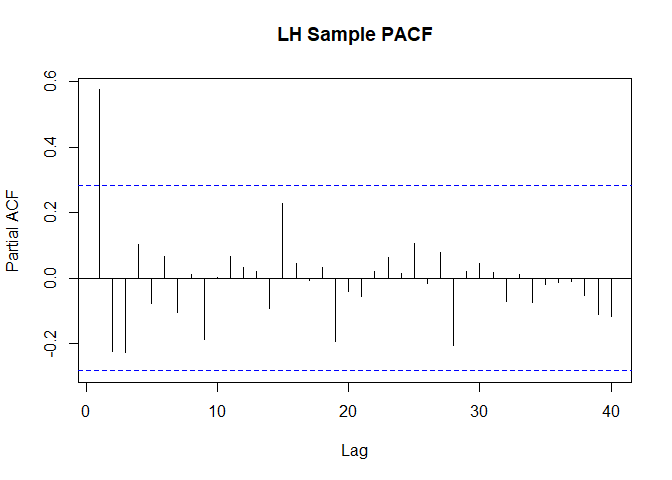
\includegraphics{LH_TS_files/figure-latex/unnamed-chunk-1-1.pdf}

As illustrated in the above plot, the partial autocorrelations appear to
``die out'' after lag=1 and remain within the confidence bounds
thereafter. This behavior is more consistent with that of an AR(1).
However, as was the case with the acf, it is also conceivable that the
series could be a moving average, if we regard the lags within the
confidence bounds as non-zero.

\section{Analyzing \& Selecting
Models}\label{analyzing-selecting-models}

In addition to full and partial autocorrelations, information criteria
was also used to select the optimal model. Aikake Information Criterion
(AIC) and Bayesian Information Criterion (BIC) assign scores to models
based on both goodness-of-fit and model complexity, with the key
difference being that BIC penalizes complexity more than AIC. The
auto.arima() function applies AIC and BIC over all possible models and
selects the model with the best (lowest) score.The function also
considers the corrected Aikake Information Criterion (\(AIC_c\)), which
also akes the sample size into account. This is important because larger
samples more accurately reflect the population than smaller samples. The
result of the function is shown below.

\begin{verbatim}
## Series: lh 
## ARIMA(1,0,0) with non-zero mean 
## 
## Coefficients:
##          ar1    mean
##       0.5739  2.4133
## s.e.  0.1161  0.1466
## 
## sigma^2 estimated as 0.2061:  log likelihood=-29.38
## AIC=64.76   AICc=65.3   BIC=70.37
\end{verbatim}

As shown above, auto.arima() recommended an AR(1) model of the form
\(x_t=0.5739x_{t-1}+2.4133\). This model was a reasonable candidate,
since an AR(1) was one of the initial classes considered based on the
ACF and PACF. Despite the results of auto.arima(), the other class
initially considered, an MA(1), was retained as a second candidate.
Aside from less favorable information criteria, there was not yet a
reason to discard this candidate. The next step was to estimate
paramters for the optimal MA(1) model and test whether any assumptions
made had been violated in either of the two candidate models. Violations
would serve as the basis for discarding a model candidate.

\section{Evaluating Model
Assumptions}\label{evaluating-model-assumptions}

The assumptions made when fitting the time series models pertain to the
model's residuals. A model's residuals are the error terms, or
differences between the modeled value and actual value of each
observation. Residuals that are overall closer to zero could thus
indicate a better fit. Residuals that are correlated or follow a clear
pattern could indicate the existance of another predictor variable that
should have been considered, which would compromise the integrity of the
model. Residual analysis is used to identify violations of the following
conditions: * The residuals are stationary and uncorrelated * The
standardized residuals are an iid sequence with mean zero and a variance
of one * The residuals are normally distributed with few outliers * The
residuals are independent

The sarima( ) function was used to estimate parameters for the optimal
model for the MA(1), the second candidate. For both model candidates,
the resulting MA(1) and the AR(1), the sarima() function was also used
for residual analysis to test the conditions delineated above. This
function outputs a time series plot, a correlogram, and a Normal Q-Q
plot for the standardized residuals to evaluate residual stationarity,
check for patterns, and assess normality. The sarima( ) output also
includes a plot for the p-values of the Ljung Box test, which tests the
null hypothesis of residual independence at each lag. In addition to
residual analysis, sarima( ) also outputs information criteria to allow
for further comparison between candidates. Finally, for each parameter
estimate, sarima( ) supplies the associated p-value, which can be used
to reject the significance of the associated term.

\begin{verbatim}
## initial  value -0.594944 
## iter   2 value -0.800449
## iter   3 value -0.800581
## iter   4 value -0.800619
## iter   5 value -0.800623
## iter   6 value -0.800623
## iter   6 value -0.800623
## final  value -0.800623 
## converged
## initial  value -0.806760 
## iter   2 value -0.806860
## iter   3 value -0.806873
## iter   4 value -0.806873
## iter   4 value -0.806873
## iter   4 value -0.806873
## final  value -0.806873 
## converged
\end{verbatim}

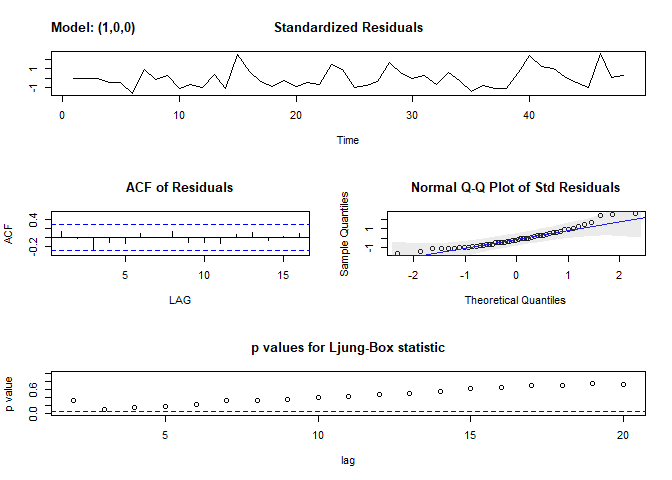
\includegraphics{LH_TS_files/figure-latex/unnamed-chunk-3-1.pdf}

\begin{verbatim}
## initial  value -0.605471 
## iter   2 value -0.763988
## iter   3 value -0.766338
## iter   4 value -0.774439
## iter   5 value -0.774775
## iter   6 value -0.774789
## iter   7 value -0.774789
## iter   7 value -0.774789
## iter   7 value -0.774789
## final  value -0.774789 
## converged
## initial  value -0.771987 
## iter   2 value -0.772013
## iter   3 value -0.772023
## iter   3 value -0.772023
## iter   3 value -0.772023
## final  value -0.772023 
## converged
\end{verbatim}

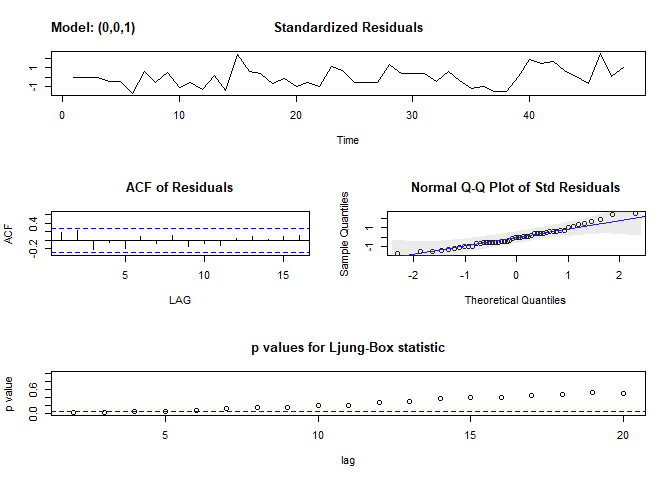
\includegraphics{LH_TS_files/figure-latex/unnamed-chunk-3-2.pdf}

For M1, the AR(1) model, residual analysis did not show that any
conditions had been violated. As illustrated in the Ljung-Box test plot,
the p-values for all Q-statistics exceeded \(\alpha=0.05\). This
indicated that that the null hypothesis need not be rejected and that
the residual independence assumption had not been violated. Conversely,
for the MA(2), the null hypothesis was rejected for the first four
Q-statistics on the basis that \(p{\leq}{\alpha}\). This meant that the
independence assumption had been violated and that the model should be
discarded.

None of the other conditions appeared to have been violated in either
model: the QQ plots \emph{largely} indicated normality, there were few
outlying standardized residuals, and the residuals appeared stationary.

Even though M2 should be discarded based on the independence assumption
violation, information criteria and mean resiudal value were used to
compare the models for additional confirmation.

\begin{center}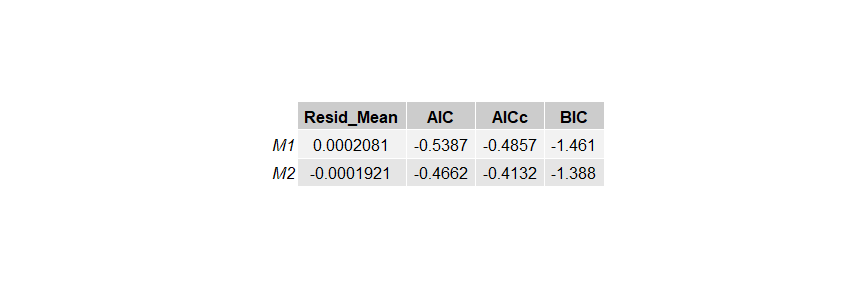
\includegraphics{LH_TS_files/figure-latex/unnamed-chunk-4-1} \end{center}

As shown in the above table, the mean residual value for both models was
close to zero. As expected, information criteria favored M1, the AR(1).

\section{Comparison to Theory \& Other
Samples}\label{comparison-to-theory-other-samples}

To further evaluate the model, the theoretical/population ACF for the
model was compared to that of the lh hormone. For further confirmation,
several random samples of the model were simulated and the ACFs were
compared to those of = the lh sample and the population. The purpose of
the simulated samples was to gain insight into how samples of the model
deviate from the population. Multiple samples were simulated before
setting the seed that produced the series plotted below.

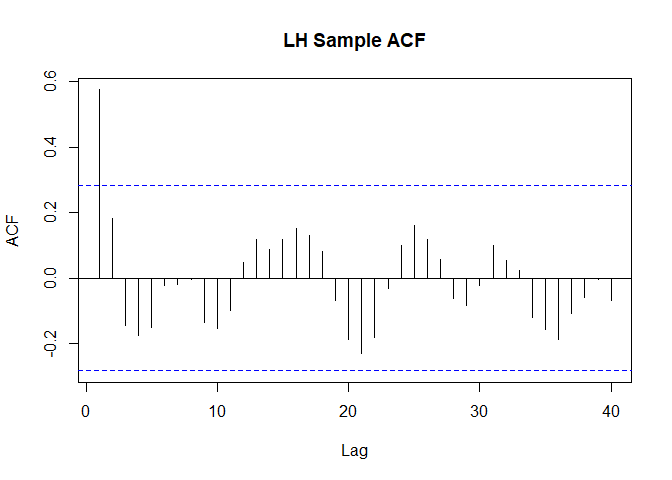
\includegraphics{LH_TS_files/figure-latex/unnamed-chunk-5-1.pdf}
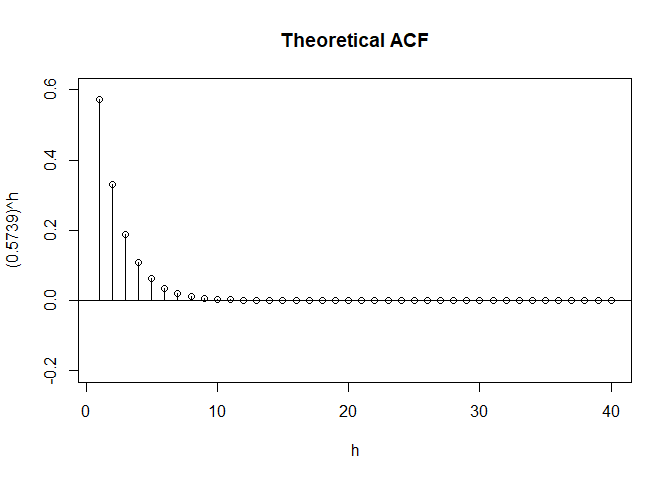
\includegraphics{LH_TS_files/figure-latex/unnamed-chunk-5-2.pdf}
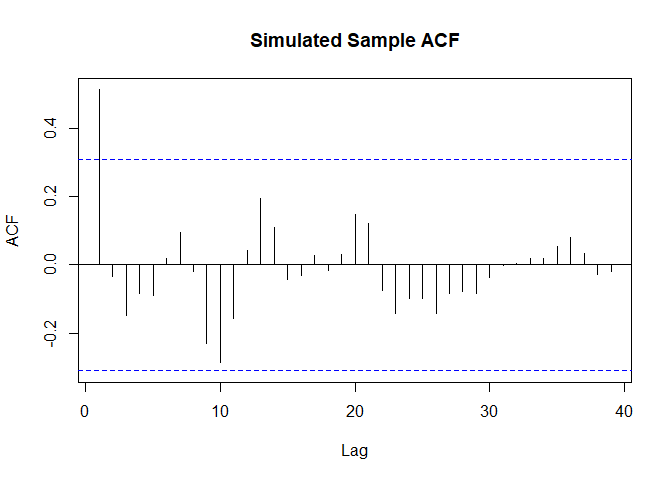
\includegraphics{LH_TS_files/figure-latex/unnamed-chunk-5-3.pdf}

\section{Conclusion}\label{conclusion}

Based on patterns observed in the sample ACF, the mangitude of
\(\hat{\phi}\), goodness-of-fit, results of residual analysis, and
resemblence to other samples of known classes, the LH sample likely a
stationary process for which an AR(1) is a very strong candidate. The
equation for the optimal AR(1) model is \(x_t=0.5739x_{t-1}+2.4133\).

In terms of forecasting, a first order autoregressive model allows for
observations to be predicted more easily, as the only input required is
the previous observation. In the context of this problem, the model
could be very useful in predicting LH levels in 10 second intervals
immediately following those taken from the female. Using only one of the
blood draws, estimates from the entire sample could be reconstructed.

Unforunately, the model's usefulness is limited by the size and time
frame of the sample upon which it was built. 48 samples were taken
within 480 seconds from one female, about whom little else is known. As
elapsed time from the last observation increases, the degree of error
for predictions also increases. Thus, the model could not be expected to
accurately predict LH levels at times that are not in the immediate
future. Additionally, the model could not be reliably applied to any
other female patient. Finally, the manner in which other factors may
impact LH levels is not known.

\section{References}\label{references}

P.J. Diggle (1990) Time Series: A Biostatistical Introduction. Oxford,
table A.1, series 3


\end{document}
